% Cyclic vs unrolled RNN — TikZ source. Compiles to a tight standalone PDF
% (pdflatex figures/unrolled-rnn.tex), which `book-scaffold build-figures`
% converts to public/figures/unrolled-rnn.svg.
%
% LEFT: one cell h <- phi(W_h h + W_x x + b), reused every step (self-loop).
% RIGHT: unrolling the loop across n tokens gives a depth-n feed-forward graph
% with TIED weights (every W_h identical, every W_x identical). The
% highlighted path x_1 -> h_1 -> h_2 -> ... -> h_n is the only route from an
% early token to a late state: it must cross every intermediate h_t.
\documentclass[tikz,border=3pt]{standalone}
\usepackage{amsmath}
\usepackage{amssymb}
\usepackage{tikz}
\usetikzlibrary{positioning,arrows.meta,calc}
\begin{document}
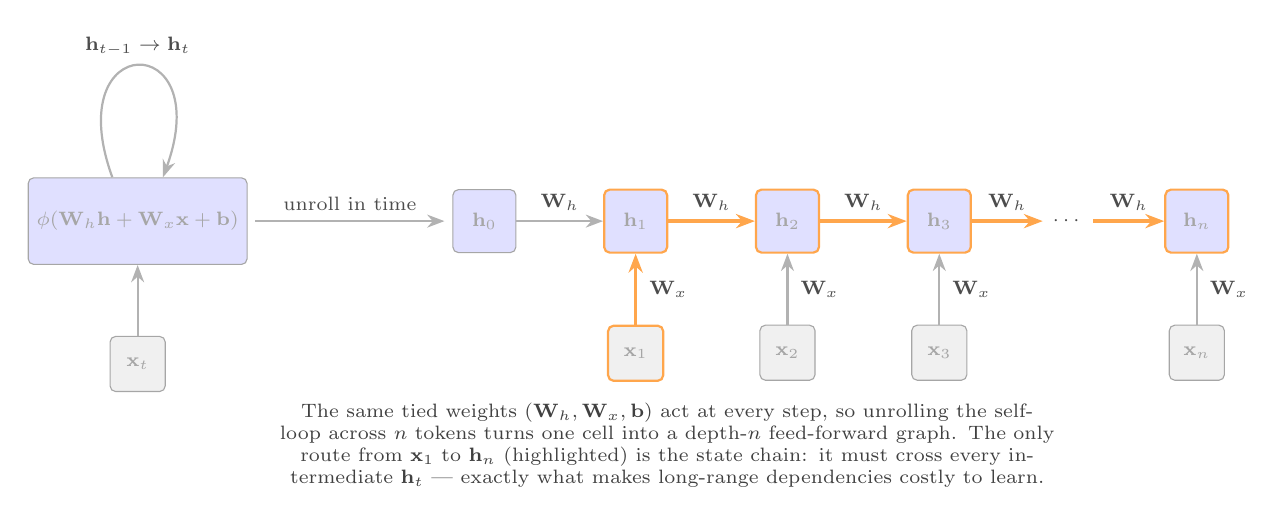
\begin{tikzpicture}[
    font=\small,
    cell/.style={draw, gray!70, rounded corners=2pt, align=center,
                 fill=blue!12, minimum height=11mm, minimum width=24mm,
                 inner sep=3pt, font=\scriptsize},
    state/.style={draw, gray!70, rounded corners=2pt, fill=blue!12,
                  minimum size=8mm, inner sep=1pt, font=\scriptsize},
    statehi/.style={state, draw=orange!70, thick},
    inp/.style={draw, gray!70, rounded corners=2pt, fill=black!6,
                minimum size=7mm, inner sep=1pt, font=\scriptsize},
    inphi/.style={inp, draw=orange!70, thick},
    op/.style={->, >={Stealth[length=2.2mm]}, gray!60, thick},
    hop/.style={->, >={Stealth[length=2.4mm]}, orange!70, very thick},
    lbl/.style={midway, above, font=\scriptsize, text=black!70},
    lblr/.style={midway, right=1pt, font=\scriptsize, text=black!70},
  ]
  % --- LEFT: cyclic (per-step) view ---
  \node[cell] (cell) {$\phi(\mathbf W_h\mathbf h+\mathbf W_x\mathbf x+\mathbf b)$};
  \draw[op] (cell.120) to[out=110,in=70,looseness=8]
    node[above, font=\scriptsize, text=black!70] {$\mathbf h_{t-1}\to\mathbf h_t$} (cell.60);
  \node[inp, below=9mm of cell.south] (xt) {$\mathbf x_t$};
  \draw[op] (xt) -- (cell.south);

  % --- divider: unroll ---
  \node[state, right=26mm of cell] (h0) {$\mathbf h_0$};
  \draw[op] ($(cell.east)+(1mm,0)$) -- ($(h0.west)+(-1mm,0)$)
    node[midway, above, font=\scriptsize, text=black!70] {unroll in time};

  % --- RIGHT: unrolled (depth-n) view ---
  \node[statehi, right=11mm of h0] (h1) {$\mathbf h_1$};
  \node[statehi, right=11mm of h1] (h2) {$\mathbf h_2$};
  \node[statehi, right=11mm of h2] (h3) {$\mathbf h_3$};
  \node[right=9mm of h3, font=\scriptsize, text=black!70] (hdots) {$\cdots$};
  \node[statehi, right=9mm of hdots] (hn) {$\mathbf h_n$};

  \draw[op]  (h0) -- (h1)     node[lbl] {$\mathbf W_h$};
  \draw[hop] (h1) -- (h2)     node[lbl] {$\mathbf W_h$};
  \draw[hop] (h2) -- (h3)     node[lbl] {$\mathbf W_h$};
  \draw[hop] (h3) -- (hdots)  node[lbl] {$\mathbf W_h$};
  \draw[hop] (hdots) -- (hn)  node[lbl] {$\mathbf W_h$};

  \node[inphi, below=9mm of h1.south] (x1) {$\mathbf x_1$};
  \node[inp,   below=9mm of h2.south] (x2) {$\mathbf x_2$};
  \node[inp,   below=9mm of h3.south] (x3) {$\mathbf x_3$};
  \node[inp,   below=9mm of hn.south] (xn) {$\mathbf x_n$};

  \draw[hop] (x1) -- (h1) node[lblr] {$\mathbf W_x$};
  \draw[op]  (x2) -- (h2) node[lblr] {$\mathbf W_x$};
  \draw[op]  (x3) -- (h3) node[lblr] {$\mathbf W_x$};
  \draw[op]  (xn) -- (hn) node[lblr] {$\mathbf W_x$};

  \node[below, align=center, text width=13cm, font=\scriptsize, text=black!75]
    at ($(cell.south)!0.5!(hn.south)+(0,-1.7)$)
    {The same tied weights $(\mathbf W_h,\mathbf W_x,\mathbf b)$ act at every step, so
     unrolling the self-loop across $n$ tokens turns one cell into a depth-$n$
     feed-forward graph. The only route from $\mathbf x_1$ to $\mathbf h_n$
     (highlighted) is the state chain: it must cross every intermediate
     $\mathbf h_t$ — exactly what makes long-range dependencies costly to learn.};
\end{tikzpicture}
\end{document}
